\documentclass[]{article}

% Imported Packages
%------------------------------------------------------------------------------
\usepackage{amssymb}
\usepackage{amstext}
\usepackage{amsthm}
\usepackage{amsmath}
\usepackage{enumerate}
\usepackage{fancyhdr}
\usepackage[margin=1in]{geometry}
\usepackage{graphicx}
\usepackage{extarrows}
\usepackage{setspace}
%------------------------------------------------------------------------------

% Header and Footer
%------------------------------------------------------------------------------
\pagestyle{plain}  
\renewcommand\headrulewidth{0.4pt}                                      
\renewcommand\footrulewidth{0.4pt}                                    
%------------------------------------------------------------------------------

% Title Details
%------------------------------------------------------------------------------
\title{IdentiSky Architectural Design}
\author{Group 2 for SFWR ENG 3A04 \\
\\ 
Alex Guerrero, guerreap, 1133763 \\
Jabrayil Malikov, malikoj, 1302641 \\
Matt Franceschini, francemj, 1310437 \\
Sam Hamel, hamels2, 1321692 \\
Vicky Bilbily, bilbilv, 1317465 \\
}
\date{March 7th, 2016}                                
%------------------------------------------------------------------------------

% Document
%------------------------------------------------------------------------------
\begin{document}

\maketitle	

\section{Introduction}
\label{sec:introduction}
% Begin Section


\subsection{Purpose}
\label{sub:purpose}
% Begin SubSection
\begin{enumerate}[a)]
	\item The purpose of this documents is to show the architecture of the system and how it will be structured.
	\item This document is to be used as a reference for the development team as well as the professor and teaching assistants of SFWR ENG 3A03. 

\end{enumerate}
% End SubSection

\subsection{System Description}
\label{sub:system_description}
% Begin SubSection
\begin{enumerate}[a)]
	\item IdentiSky is a mobile application that identifies objects in the night sky. These objects are limited to constellations and their associated stars, planets, planes, and noteable satellites. Search results are based on the user's current location, date, time, and the user's answers to questions queried by the application. 

\end{enumerate}
% End SubSection

\subsection{Overview}
\label{sub:overview}
% Begin SubSection
\begin{enumerate}[a)]

	\item Included in this document will be a couple of diagrams, one will model the functionality of system using actors
and use cases. The other will outline the use cases. There will also be an overview of the overall architectural design. 

	\item The first section will provide an brief overview of the entire document. Section 2 will provide a use case diagram for the application. The next section(section 3) will have an analysis class diagram for the application. In section 4, will be an overview of the overall architectural design of your application. Section 5 will contain the CRC cards.
	
\end{enumerate}
% End SubSection

% End Section

\section{Use Case Diagram}
\label{sec:use_case_diagram}
% Begin Section
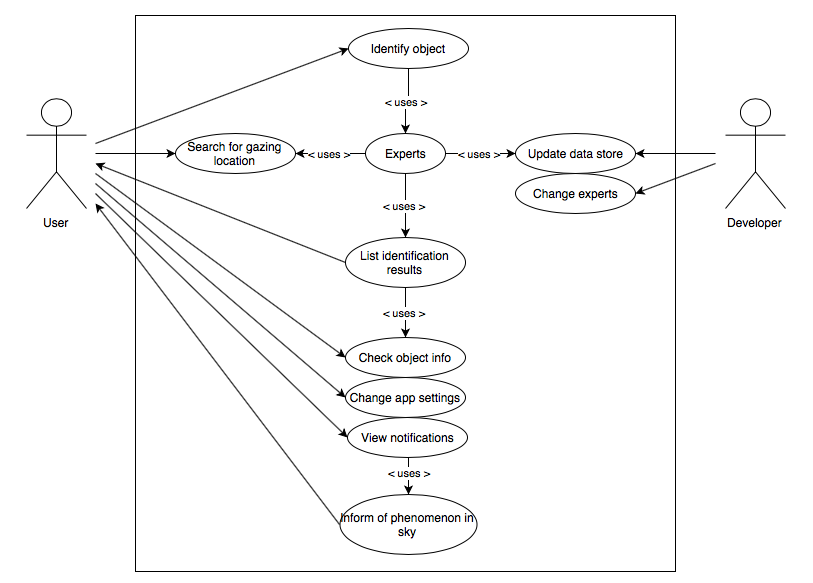
\includegraphics[scale=0.6]{UseCaseDiagram} \\
\newline
\textbf{\underline{Identify object}:} The user wants to identify an object in the sky, which prompts a questionnaire. The questionnaire gives the experts a basis to form their individual results.\\
\newline
\textbf{\underline{Experts}:} When a user requests to identify and object, experts use the information for the questionnaire to determine its identity. Experts will be mutually exclusive, each being knowledgeable on one specific and different domain. This allows for each expert to be modular and easily swappable. \\
\newline
\textbf{\underline{Search for gazing location}:} The user wants to find near by star gazing spots. The user's location is given to the expert (or experts) to determine these spots. \\
\newline
\textbf{\underline{List identification results}:} The system will display the results from the information given from the experts. When given the results from the experts, they will be filtered and ranked, only displaying the relevant information to the user. In the case of identifying an object, the top ten results will be displayed. In the case of locating star gazing spots, a map will be displayed with all the suggested points marked. The results will be within a set kilometre radius.\\
\newline
\textbf{\underline{Check object info}:} From the results of identifying an object, the user can inspect each result, revealing additional information about it. \\
\newline
\textbf{\underline{Change app settings}:} The user goes to the settings page to adjust general settings of the application, such as setting the kilometre radius for the star gazing spot search. \\
\newline
\textbf{\underline{View notifications}:} The user can check the recent notifications sent to them from the system about local sky phenomenon occurring in the near future. \\
\newline
\textbf{\underline{Inform of phenomenon in sky}:} The system sends the user notifications about local phenomenon occurring in the near future. \\
\newline
\textbf{\underline{Update data store}:} The developer wants to update the system's data store. They shall be able to add and/or removing objects as needed. \\
\newline
\textbf{\underline{Change experts}:} The developer wants to change the experts of the system. Since the experts are modular, the developer shall be add and remove them will little effort. \\
% End Section

\section{Analysis Class Diagram}
\label{sec:analysis_class_diagram}
% Begin Section
\begin{figure}[h!]
    \centering
    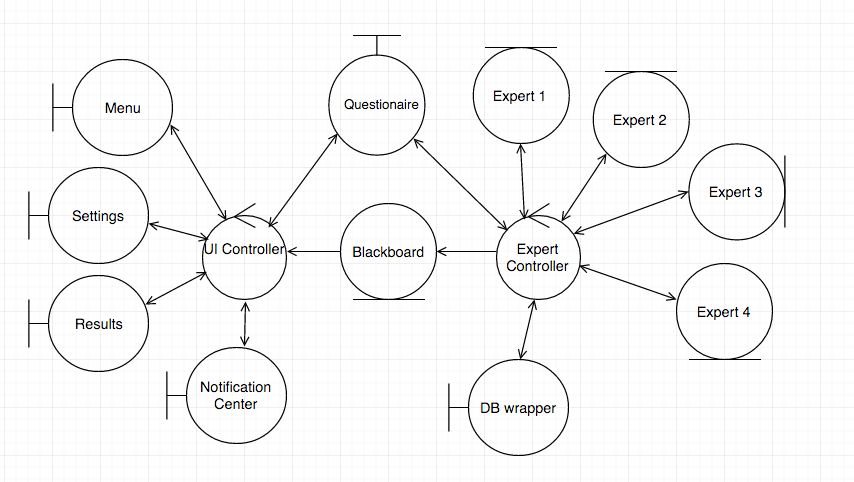
\includegraphics[scale=0.5]{analysis.png}
\end{figure}
% End Section


\section{Architectural Design}
\label{sec:architectural_design}

\subsection{System Architecture}
\label{sub:system_architecture}
% Begin SubSection

The overall architecture of IndentiSky is based off of the Blackboard Architecture Style. This architecture style is most appropriate for solving non-deterministic problems, or problems where approximate solutions are acceptable, through the collaboration of some number of distinctive, independent knowledge sources. IdentiSky fits this description, as there are many different realms of knowledge, such as date and time, location, brightness, colour, and motion, that will be considered when attempting to identify some object in the sky based on information given by the user. Since much of this information is descriptive, the application is not expected to give exact results, and estimates are appropriate. As well, depending on the category chosen by the user, different realms of knowledge may be more appropriate for finding a solution-- for example, number of stars is a useful property for identifying constellations, but nothing else. The Blackboard Architecture makes it easy to swap out knowledge sources, which is another reason that it has been selected for IdentiSky. \\

Using the Blackboard Architecture will ensure low coupling, since all knowledge sources, called \emph{experts}, will not actually communicate directly between themselves, but with the \emph{blackboard}. High cohesion is also attained, since each expert consults itself on its topic of expertise. In addition to these basic components of the Blackboard Architecture, an \emph{experts controller} will manage the experts, interfacing them with the blackboard and the \emph{data store}, and a \emph{user interface} subsystem will manage input and output between the user and the blackboard.

\begin{figure}[h!]
    \centering
    \includegraphics[scale=0.5]{architecture.png}
\end{figure}

\subsection{Subsystems}
\label{sub:subsystems}
% Begin SubSection
\begin{enumerate}
	\item User Interface
	\begin{itemize}
	    \item Purpose: 	Displays information and options to the user. Collects input data from the user.
	    \item Relationships: Sends user-information to blackboard, receives questions and results from blackboard to be displayed to the user.
	\end{itemize}
	\item Expert Controller
	\begin{itemize}
	    \item Purpose: To interface the experts, and especially to swap in (or "activate") the experts that are currently needed and swap out (or "deactivate") those that our not.
	    \item Relationships: Connects the appropriate experts to the blackboard, allowing two-way communication. Also connects each expert to the data store.
	\end{itemize}
	\item Experts
	\begin{itemize}
	    \item Purpose: Each expert's purpose is to provide a partial solution to the problem based on their particular domain of expertise.
	    \item Relationships: Gets information through the expert controller.
	\end{itemize}
	\item Blackboard
	\begin{itemize}
	    \item Purpose: To contain all the relevant information to be accessed by the experts, including information that may be added or modified by the experts.
	    \item Relationships: Gets information from the user interface and sends results and questions to the user interface. Communicates with the experts through the expert controller.
	\end{itemize}
	\item Data Store
	\begin{itemize}
	    \item Purpose: Contains all possible identifiable objects for the experts to reference.
	    \item Relationships: Accessed by the experts through the expert controller
	\end{itemize}
\end{enumerate}
% End SubSection

% End Section
	
\section{Class Responsibility Collaboration (CRC) Cards}
\label{sec:class_responsibility_collaboration_crc_cards}
% Begin Section

    \begin{table}[h!]
		\centering
		\begin{tabular}{|p{5cm}|p{5cm}|}
		\hline 
		 \multicolumn{2}{|l|}{\textbf{Class Name:} Expert Controller} \\
		\hline
		\textbf{Responsibility:} & \textbf{Collaborators:} \\\hline
		Send expert information to the Blackboard. & Expert 1-4\\
		\hline
		Send users answers to the experts & Expert 1-4, Questionnaire\\
		\hline
		\end{tabular}
	\end{table}
	
	\begin{table}[h!]
		\centering
		\begin{tabular}{|p{5cm}|p{5cm}|}
		\hline 
		 \multicolumn{2}{|l|}{\textbf{Class Name:} Expert} \\
		\hline
		\textbf{Responsibility:} & \textbf{Collaborators:} \\
		\hline
		Narrow down the identification process. & The other experts, expert controller\\
		\hline
		Access data store to cross reference user answers with known objects & Expert Controller, DB Wrapper \\
		\hline
		\end{tabular}
	\end{table}
	
	\begin{table}[h!]
		\centering
		\begin{tabular}{|p{5cm}|p{5cm}|}
		\hline 
		 \multicolumn{2}{|l|}{\textbf{Class Name:} Blackboard} \\
		\hline
		\textbf{Responsibility:} & \textbf{Collaborators:} \\\hline
		Determine what the object could be. & Expert Controller, Expert 1-4\\
		\hline
		Compile all of the expert input and determine which of the answers is the most likely & Expert Controller, Expert 1-4, Questionnaire\\
		\hline
		Send the compiled answer to the user & UI Controller \\
		\hline
		\end{tabular}
	\end{table}
	
	\begin{table}[h!]
		\centering
		\begin{tabular}{|p{5cm}|p{5cm}|}
		\hline 
		 \multicolumn{2}{|l|}{\textbf{Class Name:} Questionnaire} \\
		\hline
		\textbf{Responsibility:} & \textbf{Collaborators:} \\\hline
		Send questions for the user to answer & UI Controller\\
		\hline
		Send users answers to the experts & Expert Controller \\
		\hline
		\end{tabular}
	\end{table}
	
	\begin{table}[h!]
		\centering
		\begin{tabular}{|p{5cm}|p{5cm}|}
		\hline
		 \multicolumn{2}{|l|}{\textbf{Class Name:} DB Wrapper} \\
		\hline
		\textbf{Responsibility:} & \textbf{Collaborators:} \\\hline
		Allow access to data stores for each expert. Only the expert which is associated with each data store can access it & Expert Controller\\
		\hline
	    Encrypts the communications of the app and the data stores. & \\
		\hline
		\end{tabular}
	\end{table}
	
	\begin{table}[h!]
		\centering
		\begin{tabular}{|p{5cm}|p{5cm}|}
		\hline 
		 \multicolumn{2}{|l|}{\textbf{Class Name:} UI Controller} \\
		\hline
		\textbf{Responsibility:} & \textbf{Collaborators:} \\\hline
		Controls the interaction with the user & \\
		\hline
	    Takes the user input and sends it the correct place & \\
		\hline
		Displays the questions to be answered to aid in the identification process & Questionnaire \\
		\hline
		Display the answer(s) that the experts have come up with & Blackboard, Results \\
		\hline
		\end{tabular}
	\end{table}
	
	\begin{table}[h!]
		\centering
		\begin{tabular}{|p{5cm}|p{5cm}|}
		\hline 
		 \multicolumn{2}{|l|}{\textbf{Class Name:} Notification Center} \\
		\hline
		\textbf{Responsibility:} & \textbf{Collaborators:} \\\hline
		Send push notifications to the user to alert them of cool things they can see in the sky based on their location & Location Expert, UI Controller\\
		\hline
		\end{tabular}
	\end{table}
	
	\begin{table}[h!]
		\centering
		\begin{tabular}{|p{5cm}|p{5cm}|}
		\hline 
		 \multicolumn{2}{|l|}{\textbf{Class Name:} Results} \\
		\hline
		\textbf{Responsibility:} & \textbf{Collaborators:} \\\hline
		Displays the results from the experts & Blackboard, UI Controller\\
		\hline
		\end{tabular}
	\end{table}
	
	\begin{table}[h!]
		\centering
		\begin{tabular}{|p{5cm}|p{5cm}|}
		\hline 
		 \multicolumn{2}{|l|}{\textbf{Class Name:} Settings} \\
		\hline
		\textbf{Responsibility:} & \textbf{Collaborators:} \\\hline
		Allows user to filter what they want to find & UI controller\\
		\hline
		Allows user to change general settings & UI Controller \\
		\hline
		\end{tabular}
	\end{table}
	
	\begin{table}[h!]
		\centering
		\begin{tabular}{|p{5cm}|p{5cm}|}
		\hline 
		 \multicolumn{2}{|l|}{\textbf{Class Name:} Menu} \\
		\hline
		\textbf{Responsibility:} & \textbf{Collaborators:} \\\hline
		Displays at the app startup with prompts for what the user wants to do next & UI Controller\\
		\hline
		\end{tabular}
	\end{table}
% End Section

\end{document}